
\section{Shape of a dusty radiative bow wave}
\label{sec:shape-dust-wave}

\begin{figure}
  \centering
  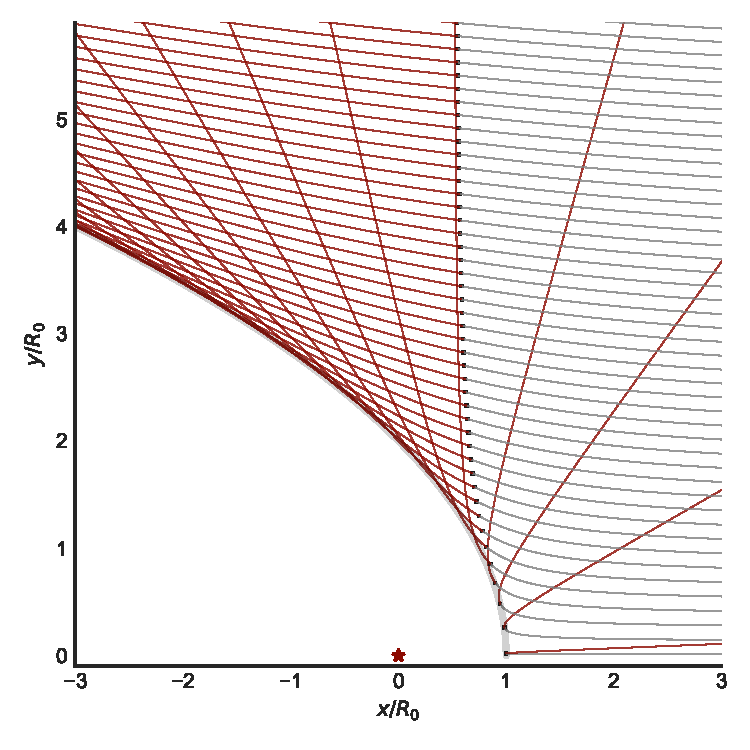
\includegraphics[width=\linewidth]{figs/dust-trajectories}
  \caption[Dust grain trajectories]{Dust grain trajectories under
    influence of a repulsive central \(r^{-2}\) radiative force.  Dust
    grains approach from the right at a uniform velocity and with a
    variety of impact parameters (initial \(y\)-coordinate). The
    central source is marked by a red star at the origin, and its
    radiative force deflects the trajectories into a hyperbolic shape,
    each of which reaches a minimum radius marked by a small black
    square.  The incoming hyperbolic trajectories are traced in gray
    and the outgoing trajectories are traced in red.  The locus of
    closest approach of the outgoing trajectories is parabolic in
    shape (traced by the thick, light gray line) and this constitutes
    the inner edge of the bow wave. }
  \label{fig:dust-trajectories}
\end{figure}


%%% Local Variables:
%%% mode: latex
%%% TeX-master: "quadrics-bowshock"
%%% End:
